\documentclass[twoside,a4paper]{uva-bachelor-thesis}
% Add openright for final thesis

% Define this when starting to use the template:
\def\course{Masterproject Software Engineering}
\def\courseshort{Masterproject SE}
\def\assignment{Thesis Proposal}
\def\name{Interaction Design for Fragment-based Molecule Parameterisation}
\def\auth{Jimi M. van der Woning}
\def\duedate{\today}
%\def\org{CWI: Life Sciences and SWAT groups}
\def\supervis{
    \begin{tabular}{lll}
    Mohammed El-Kebir & Gunnar W. Klau & Tijs van der Storm \\
    CWI: Life Sciences & CWI: Life Sciences & CWI: SWAT \\
    \url{M.El-Kebir@cwi.nl} & \url{G.W.Klau@cwi.nl} & \url{T.van.der.Storm@cwi.nl} \\
    Room M278 & Room M276 & Room L225
    \end{tabular}}
% The document is now set correctly

\usepackage{graphicx}
\usepackage{wrapfig}
\usepackage{caption}
\usepackage{subcaption}
\usepackage{multirow}
\usepackage{url}
\usepackage{listings}
\usepackage{verbatim}
\usepackage{lipsum}

\usepackage{fancyhdr}
\usepackage[colorlinks, linkcolor=black, urlcolor=black, citecolor=black]{hyperref}
\usepackage{fancyhdr}
\setlength{\headheight}{15pt}

% Improve the lipsum package by automatically showing the next lipsum
\newcounter{LipsumCounter}
\setcounter{LipsumCounter}{1}
\newcommand{\nlipsum}{\lipsum[\value{LipsumCounter}] \addtocounter{LipsumCounter}{1}}

% Nicer labels and references for chapters, sections and figures
\newcommand{\archref}[2]{\hyperref[#2]{#1}}
\newcommand{\chlab}[1]{\label{chapter:#1}}
\newcommand{\chref}[1]{\archref{chapter~\ref{chapter:#1}}{chapter:#1}}
\newcommand{\Chref}[1]{\archref{Chapter~\ref{chapter:#1}}{chapter:#1}}
\newcommand{\seclab}[1]{\label{section:#1}}
\newcommand{\secref}[1]{\archref{section~\ref{section:#1}}{section:#1}}
\newcommand{\Secref}[1]{\archref{Section~\ref{section:#1}}{section:#1}}
\newcommand{\figlab}[1]{\label{figure:#1}}
\newcommand{\figref}[1]{\archref{figure~\ref{figure:#1}}{figure:#1}}
\newcommand{\Figref}[1]{\archref{Figure~\ref{figure:#1}}{figure:#1}}

% Chapter and page storage
\def \CurrChapter {}
\def \LastSection {}
\def \CurrSection {}
\newcounter{CurrPage}
\setcounter{CurrPage}{0}

\pagestyle{fancy} 
\renewcommand{\markboth}[2]{\def \CurrChapter {#1}} % For use with \tableofcontents
\renewcommand{\chaptermark}[1]{\def \CurrChapter {#1} \def \CurrSection {}}
\renewcommand{\sectionmark}[1]{ %
  \ifthenelse{ %
    \equal{\thepage}{\value{CurrPage}} %
  } %
  {\def \CurrSection {: #1}} %
  {\let \LastSection \CurrSection \def \CurrSection {: #1} \setcounter{CurrPage}{\value{page}}} %
}

% Headers and footers
\renewcommand{\footrulewidth}{0.5pt}

\fancyhf{}
\fancyfoot[LE,RO]{\textit{\thepage}}
\fancyfoot[RE,LO]{\textit{\auth}}
\fancyhead[RE,LO]{\textit{\courseshort: \assignment}}
\fancyhead[LE,RO]{ %
  \ifthenelse{ %
    \equal{\thepage}{\value{CurrPage}} %
  } %
  {\textit{\nouppercase{\CurrChapter\LastSection}}} %
  {\let \LastSection \CurrSection \textit{\nouppercase{\CurrChapter\LastSection}}} %
}

\fancypagestyle{plain}{ %
\fancyhf{} %
\fancyfoot[LE,RO]{\textit{\thepage}} %
\fancyfoot[RE,LO]{\textit{\auth}} %
\renewcommand{\headrulewidth}{0pt} % remove lines as well
}

\setlength{\parskip}{.5em}

\title{\course}
\subtitle{\assignment}
\subsubtitle{\name}
\author{Jimi M. van der Woning\\
        \url{Jimi.vanderWoning@student.uva.nl}\\
        Student ID 6061400
        }
%\organization{\org}
\supervisors{\supervis}

\begin{document}
\maketitle

% More vertical spacing in tables
\renewcommand*\arraystretch{1.5}

\setlength{\parskip}{0px}
\tableofcontents
\setlength{\parskip}{.5em}

\chapter{Project summary}
\chlab{summary}

In the world of biomolecular science, molecular simulations are gaining in importance. These simulations are used to study biomolecular systems at an atomic level such that interactions between molecules can be analysed. To perform these simulations, a set of parameters is needed, including the atomic partial charges of a molecule. Calculating these charges, however, can take a lot of time, even on advanced computation clusters.

As it is seemingly impossible to speed up the partial charge calculations, an alternative way to retrieve them should be developed. It is known that similar sections in two different molecules often have roughly the same atomic charges. Therefore, it should be possible to assign the charges of a molecule based on the known charges of sections of other molecules.

Finding the best matches is something only humans (read: experienced scientists) can do. Therefore, a tool needs to be designed that allows them to visualise a molecule and a set of related sections of other molecules. They should be able to pick the best matches and assign their atomic charges to the molecule that is being analysed. The tool should also allow for manual adjustment of the charges, as these are never exactly the same in other molecules.

This project aims to answer the following research questions:
\begin{itemize}
\item How can chemists interact with a tool for assigning partial atomic charges, based on those of similar sections in other molecules?
\item Is it feasible to do manual partial charge assignment in a reasonable amount of time?
\item Compared to computed partial charges, how well can manual atomic charge assignment be done?
\end{itemize}

\chapter{Problem analysis}

Biomolecular simulations are becoming increasingly important for drug development. In these simulations, force field models are required to describe the interatomic relations of the drug molecules. Often used force field models include \verb|AMBER|, \verb|CHARMM|, \verb|GROMACS|, \verb|GROMOS| and \verb|OPLS|. In order to run a simulation. These force fields require a certain topology. This topology should include the atom types, bonds, angles, atomic charges and charge group assignments.

Figure \ref{fig:partial_charges} shows the topology of a nitroethane molecule. Here, every oval symbolises an atom. The atom type is the letter on the top rule of the oval, i.e. \verb|H| is the atom type of the sphere \verb|H5 (6)|. The first number indicates the index in the list of atoms of that type (\verb|5| in the example), the second the overall atom index in the molecule (\verb|6| in the example). The bonds between atoms are shown as lines between the ovals and the atomic charges are given by the number at the bottom row of the oval (\verb|0.071| for \verb|H5 (6)|). Finally, the colouring of the atoms and the squares around them denote a molecular charge group. These are groups of connected atoms, for which the total charge is ideally equal to that of the whole molecule.

\begin{figure}[h!]
\begin{center}
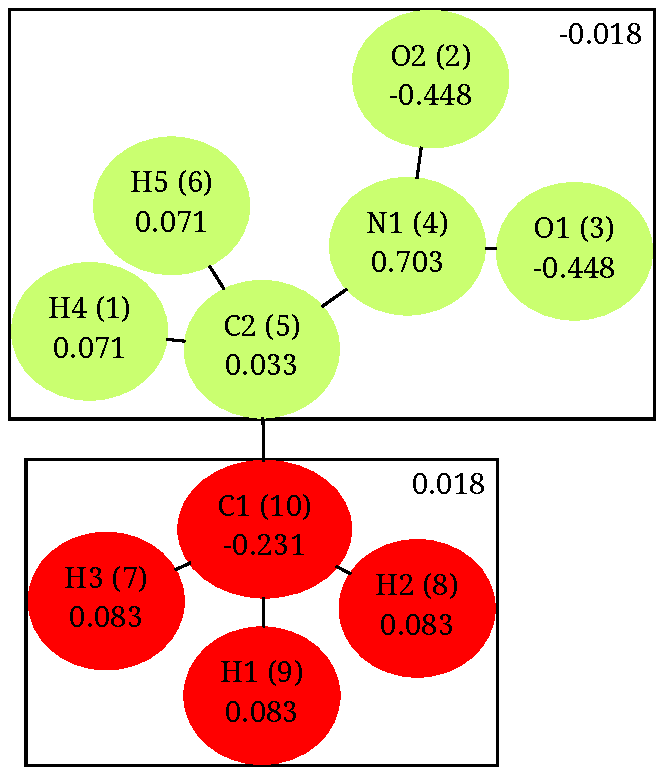
\includegraphics[width=.4\textwidth]{img/partial_charges.pdf}
\caption{Topology of nitroethane ($C_{2}H_{5}NO_{2}$).}
\label{fig:partial_charges}
\end{center}
\end{figure}

In a recent study, El-Kebir, Klau et al. have developed an algorithm that allows for fast and reasonable assignment of charge groups~\cite{canzar2012charge}. As this is now optimized, they focuss on a different step in the parameterization, that of calculating the atomic partial charges. % TODO: etc


Here you present your analysis of the problem situation that your research will address. How does this problem manifest itself at your host organization? Also summarizes existing scientific insight into the problem (result of your literature survey, see below).

\lipsum[5]


\chapter{Research methods}
\chlab{methods}

The main question that this research project will try to answer is the following:
\begin{quote}
How can chemists best interact with a tool for fragment-based molecule parameterisation, such that this yields results of comparable quality to conventional methods, while being done faster?
\end{quote}
In order to answer this question, such tool will be designed and a prototype of it will be implemented. User studies will be conducted to evaluate the tool's design and results. In those studies, the results obtained by using the tool will be compared to those obtained using conventional methods, i.e. complex quantum mechanical calculations~(see~\chref{problems}).


\section{The tool}
\seclab{tool}

% TODO: why web?!
The requirements of the molecule parameterisation tool have been specified in \chref{problems}. It has been decided to implement the tool in \verb|HTML5| and \verb|JavaScript|, which allows for great portability and availability across different operating systems and platforms. It also makes the tool future-proof, by following the current trend of bringing everything to the web.

Not surprisingly, there are no existing tools for fragment-based molecule parameterisation, as this is a new concept. Furthermore, no tools exist for comparing molecules - or fragments of them - either. What does exist is a wide range of tools and programs for showing and editing molecules. This includes stand-alone molecule drawing software such as \verb|Accelerys Draw|~\cite{accelrys2012accelrys} and \verb|Avogadro|~\cite{hanwell2012avogadro}, two-dimensional web-based molecule editors like \verb|ChemDoodle 2D Sketcher|~\cite{ichemlabs2013chemdoodle}, \verb|Molsoft HTML5 Molecule Editor|~\cite{molsoft2012molsoft} and \verb|Marvin for JavaScript|~\cite{chemxon2013marvin}, and online three-dimensional visualisation tools \verb|JSMol|~\cite{hanson2013jsmol} and \verb|CanvasMol|~\cite{altered2013canvasmol}.

These existing tools will serve as an initial guideline for the tool to be developed, and parts of their implementations may be reused. The rest of the tool, however, will need to be designed and developed from scratch. The design will follow the basic interaction design principles as posed by Norman and others~(see \secref{id_principles}), the knowledge about learing~(see \secref{id_learning}), and keep in mind the insights gained by the developers of other molecule software~(see \secref{software}).

As there is no existing software for fragment-based molecule parameterisation, there is also no baseline to which the developed tool can be compared. In order to still be able to say something about the quality of the tool, two different implementations of it will be made. There are a few axles along which this difference can be made. It could, for instance, be possible to compare the results obtained by two implementations that have a different way of visualising molecules. Visualising molecules, however, is a well-exhausted field of research, leaving very little room for new ideas.

\begin{figure}[h!]
\begin{center}
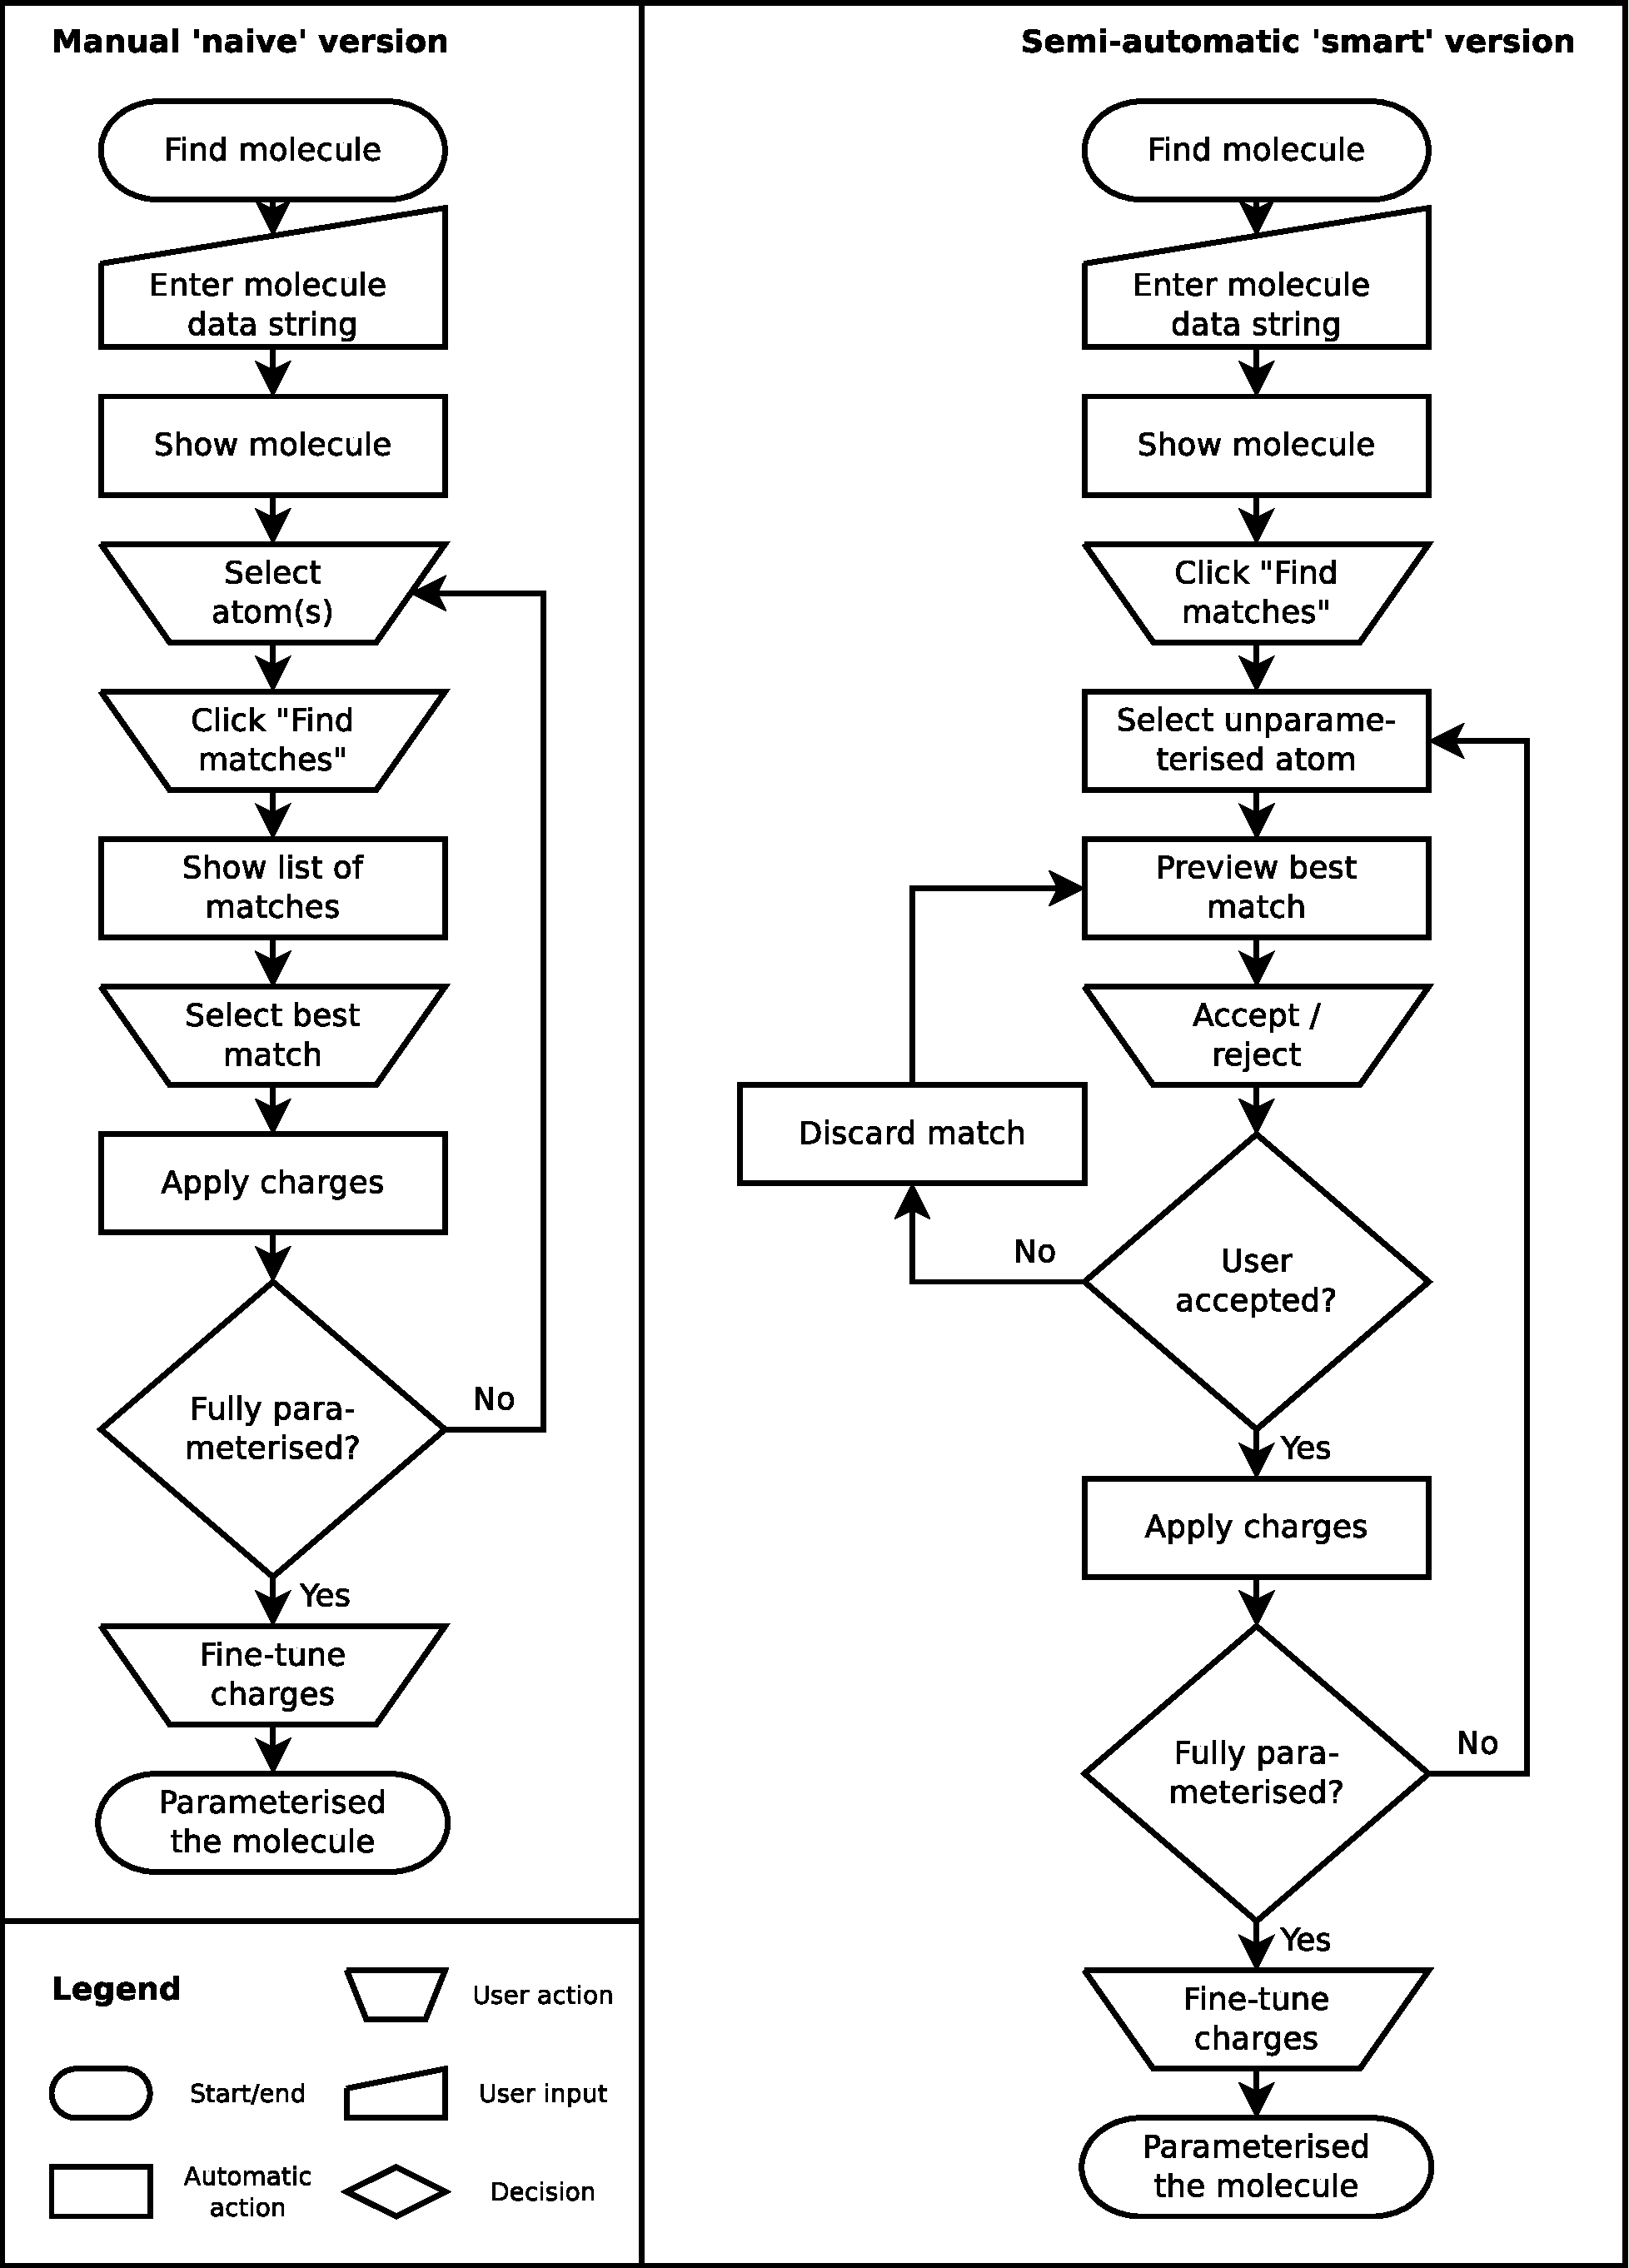
\includegraphics[width=.9\textwidth]{img/complete_id.pdf}
\caption{The two different interaction designs.}
\figlab{id_flows}
\end{center}
\end{figure}

%\begin{figure}[h!]
%\begin{subfigure}[t]{0.35\textwidth}
%\centering
%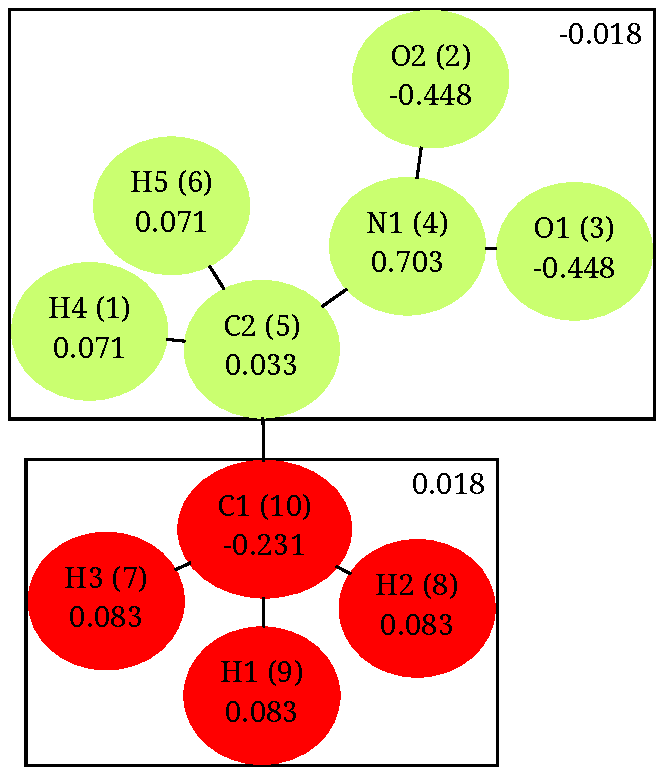
\includegraphics[width=100px]{img/partial_charges.pdf}
%\caption{The manual `naive' version.}
%\figlab{manual_id}
%\end{subfigure}\\
%\begin{subfigure}[t]{0.35\textwidth}
%\centering
%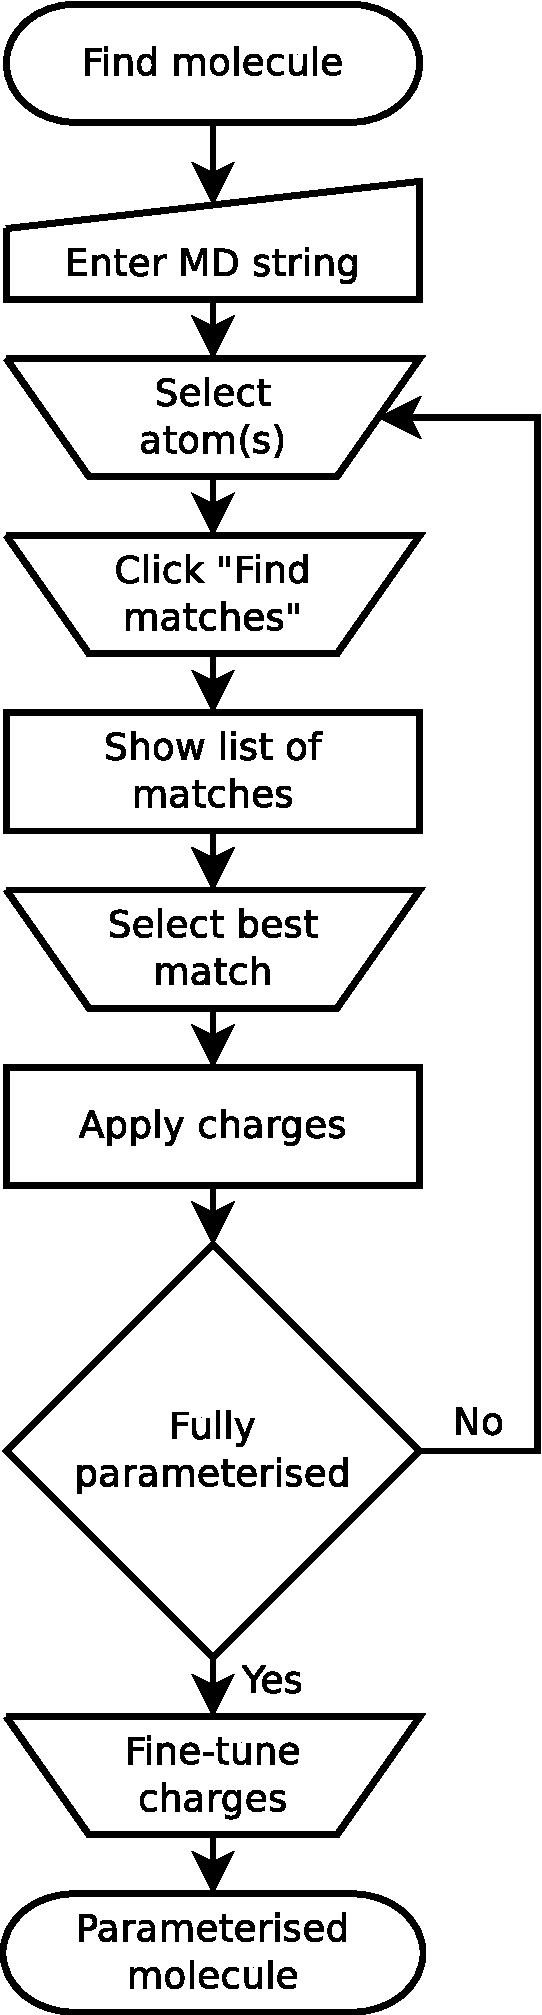
\includegraphics[width=123px]{img/manual_id.pdf}
%\caption{The manual `naive' version.}
%\figlab{manual_id}
%\end{subfigure}
%\begin{subfigure}[t]{0.65\textwidth}
%\centering
%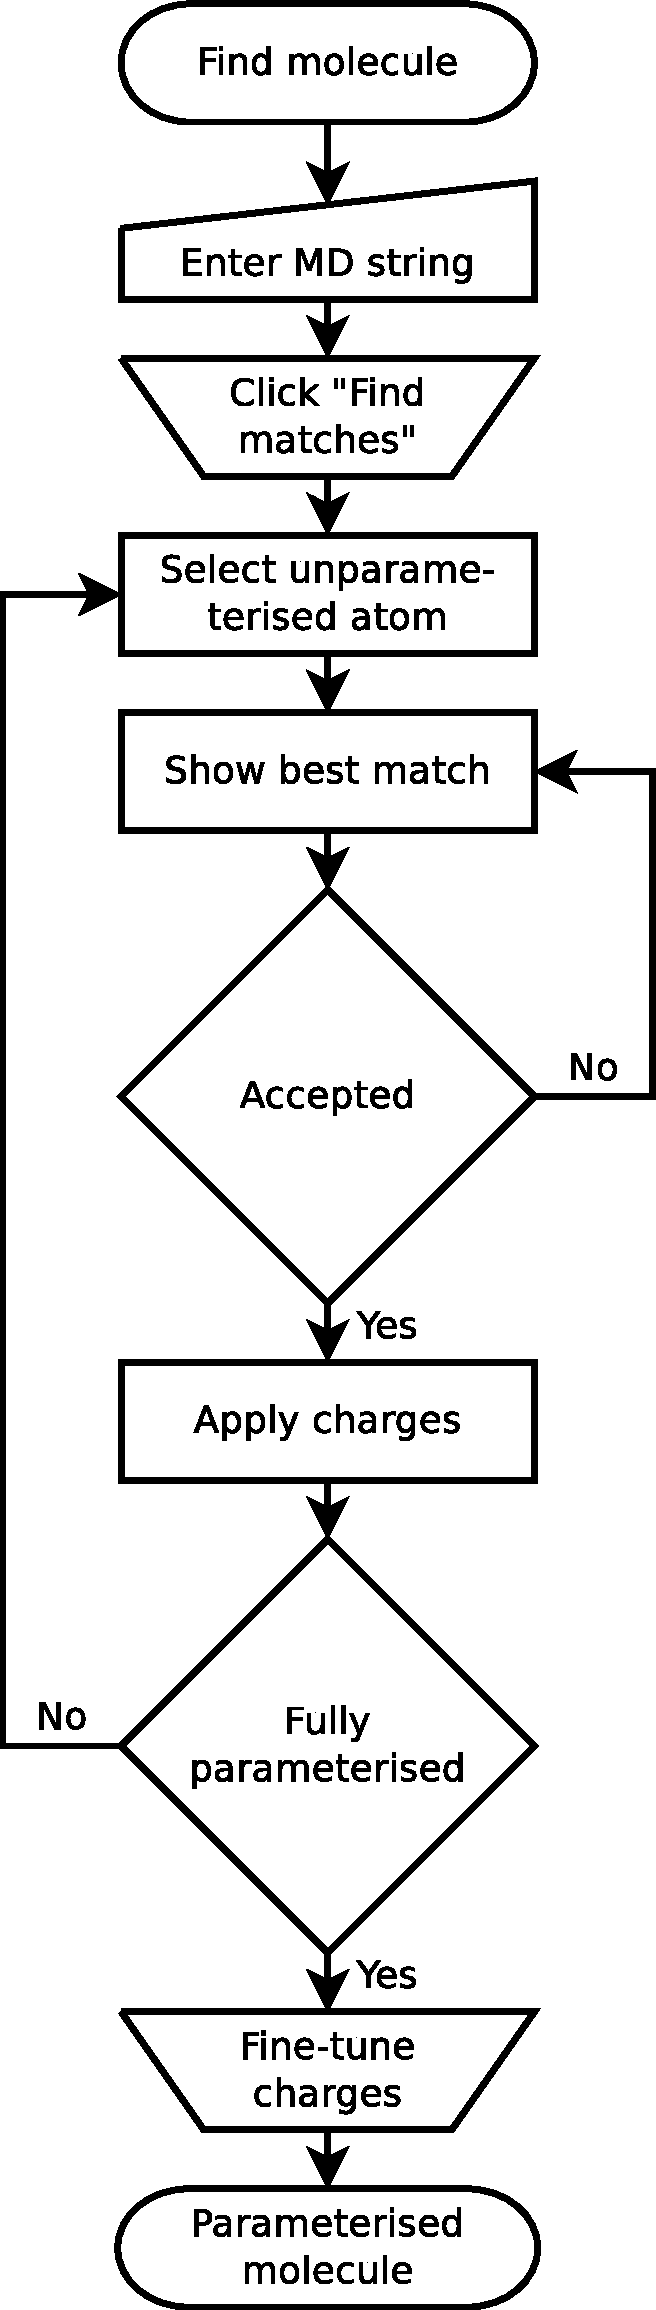
\includegraphics[width=220px]{img/semiauto_id.pdf}
%\caption{The semi-automatic `smart' version.}
%\figlab{semiauto_id}
%\end{subfigure}
%\caption{The two different interaction designs.}
%\figlab{id_flows}
%\end{figure}

Another possible variable in the tool is the way its users will interact with it and especially its degree of automation. Varying this degree has been the subject of several studies~(e.g.~\cite{payne2000varying, horvitz1999principles, marcus1987taking, norman1990problem}, see also \secref{id_automation}), all of which concluded the degree to which automation can be applied is highly dependent on the context of the system and sometimes even to the situation in which the system is used.

When implementing multiple versions of a tool with different levels of interaction, it is often decided to make three versions: a `naive' version without much automation, a `cooperative' version in which the user is given advise, and an `autonomous' version that only requires some parameterisation~(see~\cite{payne2000varying} and \secref{id_automation}). As it is considered hard to parameterise a molecule based on fragments of other molecules and little is known on what is the best way of doing this, an autonomous version of a tool that does this cannot yet be developed. The other two versions, however, seem to be perfectly implementable and both can be considered useful.

\Figref{id_flows} shows a naive and a cooperative interaction design for the tool that will be developed. Here, the cooperative design has been called the `smart' version to accentuate its differences with the naive version. The following sections will discuss these two interaction designs, the motivation behind them, their workings, and the hypotheses about them.

\subsection{Manual `naive' version}
In the naive version of the tool, the following steps should be followed to fully parameterise a molecule:
\begin{enumerate}[itemsep=.1em, parsep=.2em, topsep=0em]
\item The user enters a molecule data string (in \verb|SMILES|, \verb|InChI|, or other format);
\item The user selects a single atom or a set of \emph{connected} atoms;
\item The user clicks the ``Find matches'' button;
\item A list of matching fragments will be shown, ordered such that the highest rated match comes first and the lowest last. The user can browse through them, preview the result of selecting that match and, once he has found what he sees as the best match, select this match. Hereafter, the charges from that match will be assigned to the molecule;
\item
\begin{itemize}[leftmargin=0cm, itemsep=.1em, parsep=.1em]
\item[]{\bf Unparameterised atoms remain}:\\The user selects another atom / list of connected atoms. Back to step 3;
\item[] {\bf Molecule fully parameterised}:\\Continue to step 6;
\end{itemize}
\item When needed, the user can fine-tune the atom charges by selecting an atom and modifying its charge using an input field. In order to assist him in this process, the fragments that were matched to this atom \emph{and} have been selected will be shown;
\item The user is done.
\end{enumerate}

\noindent
In the matching process, it is possible that an already charged atom is present in another chosen fragment. In the case where these charges differ, the user will be asked to choose what should happen, which can be one of:
\begin{enumerate}[itemsep=.1em, parsep=.2em, topsep=0em]
\item Take the average of the two charges;
\item Keep the current value;
\item Take the new value;
\item Manually enter a value.
\end{enumerate}

\subsection{Semi-automatic `smart' version}
Using the semi-automatic version of the tool, the user should follow the following steps on order to fully parameterise a molecule:
\begin{enumerate}[itemsep=.1em, parsep=.2em, topsep=0em]
\item The user enters a molecule data string (in SMILES, InChI, or other format);
\item The user clicks the ``Find matches'' button. One of the atoms will now be automatically selected and matching fragments will be retrieved;
\item The highest rated match is previewed on the molecule. The user can either accept or reject this proposed match;
\item
\begin{itemize}[leftmargin=0cm, itemsep=.1em, parsep=.1em]
\item[]{\bf Rejected}:\\Remove this match from the list of matching fragments (the user \emph{can} go back to this one if he changes his mind). Back to step 3;
\item[] {\bf Accepted}:\\Assign the charges of the fragment to the molecule. Continue to step 5;
\end{itemize}
\item
\begin{itemize}[leftmargin=0cm, itemsep=.1em, parsep=.1em]
\item[]{\bf Unparameterised atoms remain}:\\Another unparameterised atom is automatically selected and similar fragments are retrieved. Back to step 3;
\item[] {\bf Molecule fully parameterised}:\\Continue to step 6;
\end{itemize}
\item The user can now fine-tune the charges by selecting an atom and modifying the charge using some input field, if he wants to do so. In order to assist him in this process, suggestions will be given on what atoms to fine-tune and to what value they should be adjusted;
\item The user is done.
\end{enumerate}

\noindent
In the matching process, it is possible that an already charged atom is present in another chosen fragment. In the case where these charges differ, the atom's charge will be automatically calculated from the two charges. Experimentation has yet to show the best way to do this, but, presumably, taking the average of the two will be a good solution.


\subsection{Pros and cons}
Both of the previously discussed methods have their benefits and disadvantages. Because of the limited level of user interaction in the `smart' version, parameterising a molecule can presumably be done much faster than in the `naive'  version. However, it is questionable how good the parameterisation will be, as the user is not really encouraged to explore a whole lot of fragments. Even though he will always be presented the highest rated match first, this match will not always be the best one. If, however, the user \emph{does} want to explore some other fragments, this might take more time than in the naive version, as only one fragment can be shown at a time.

The naive version may take up more time than the smart version, but it \emph{does} allow for a much higher level of control. The user can easily decide what atoms should be parameterised at which time and has a clear overview of the matching fragments. Furthermore, he can manually decide what should happen with overlapping fragments and can modify atom charges at any point in the process. If, however, the user lacks the experience of how to parameterise a molecule, or does not know what he is doing, he may not be able to make the right decisions, or even get lost in the large set of options. As the tool is aimed to be used by experienced scientists only, this should not be a problem, but experimentation will need to confirm that.


\section{Hypotheses}
\seclab{hypotheses}
Blah blah Brehmer and Munzer typololy, blahblah differences, blahblah \figref{id_typologies}\ldots

\begin{sidewaysfigure}[p]
\begin{center}
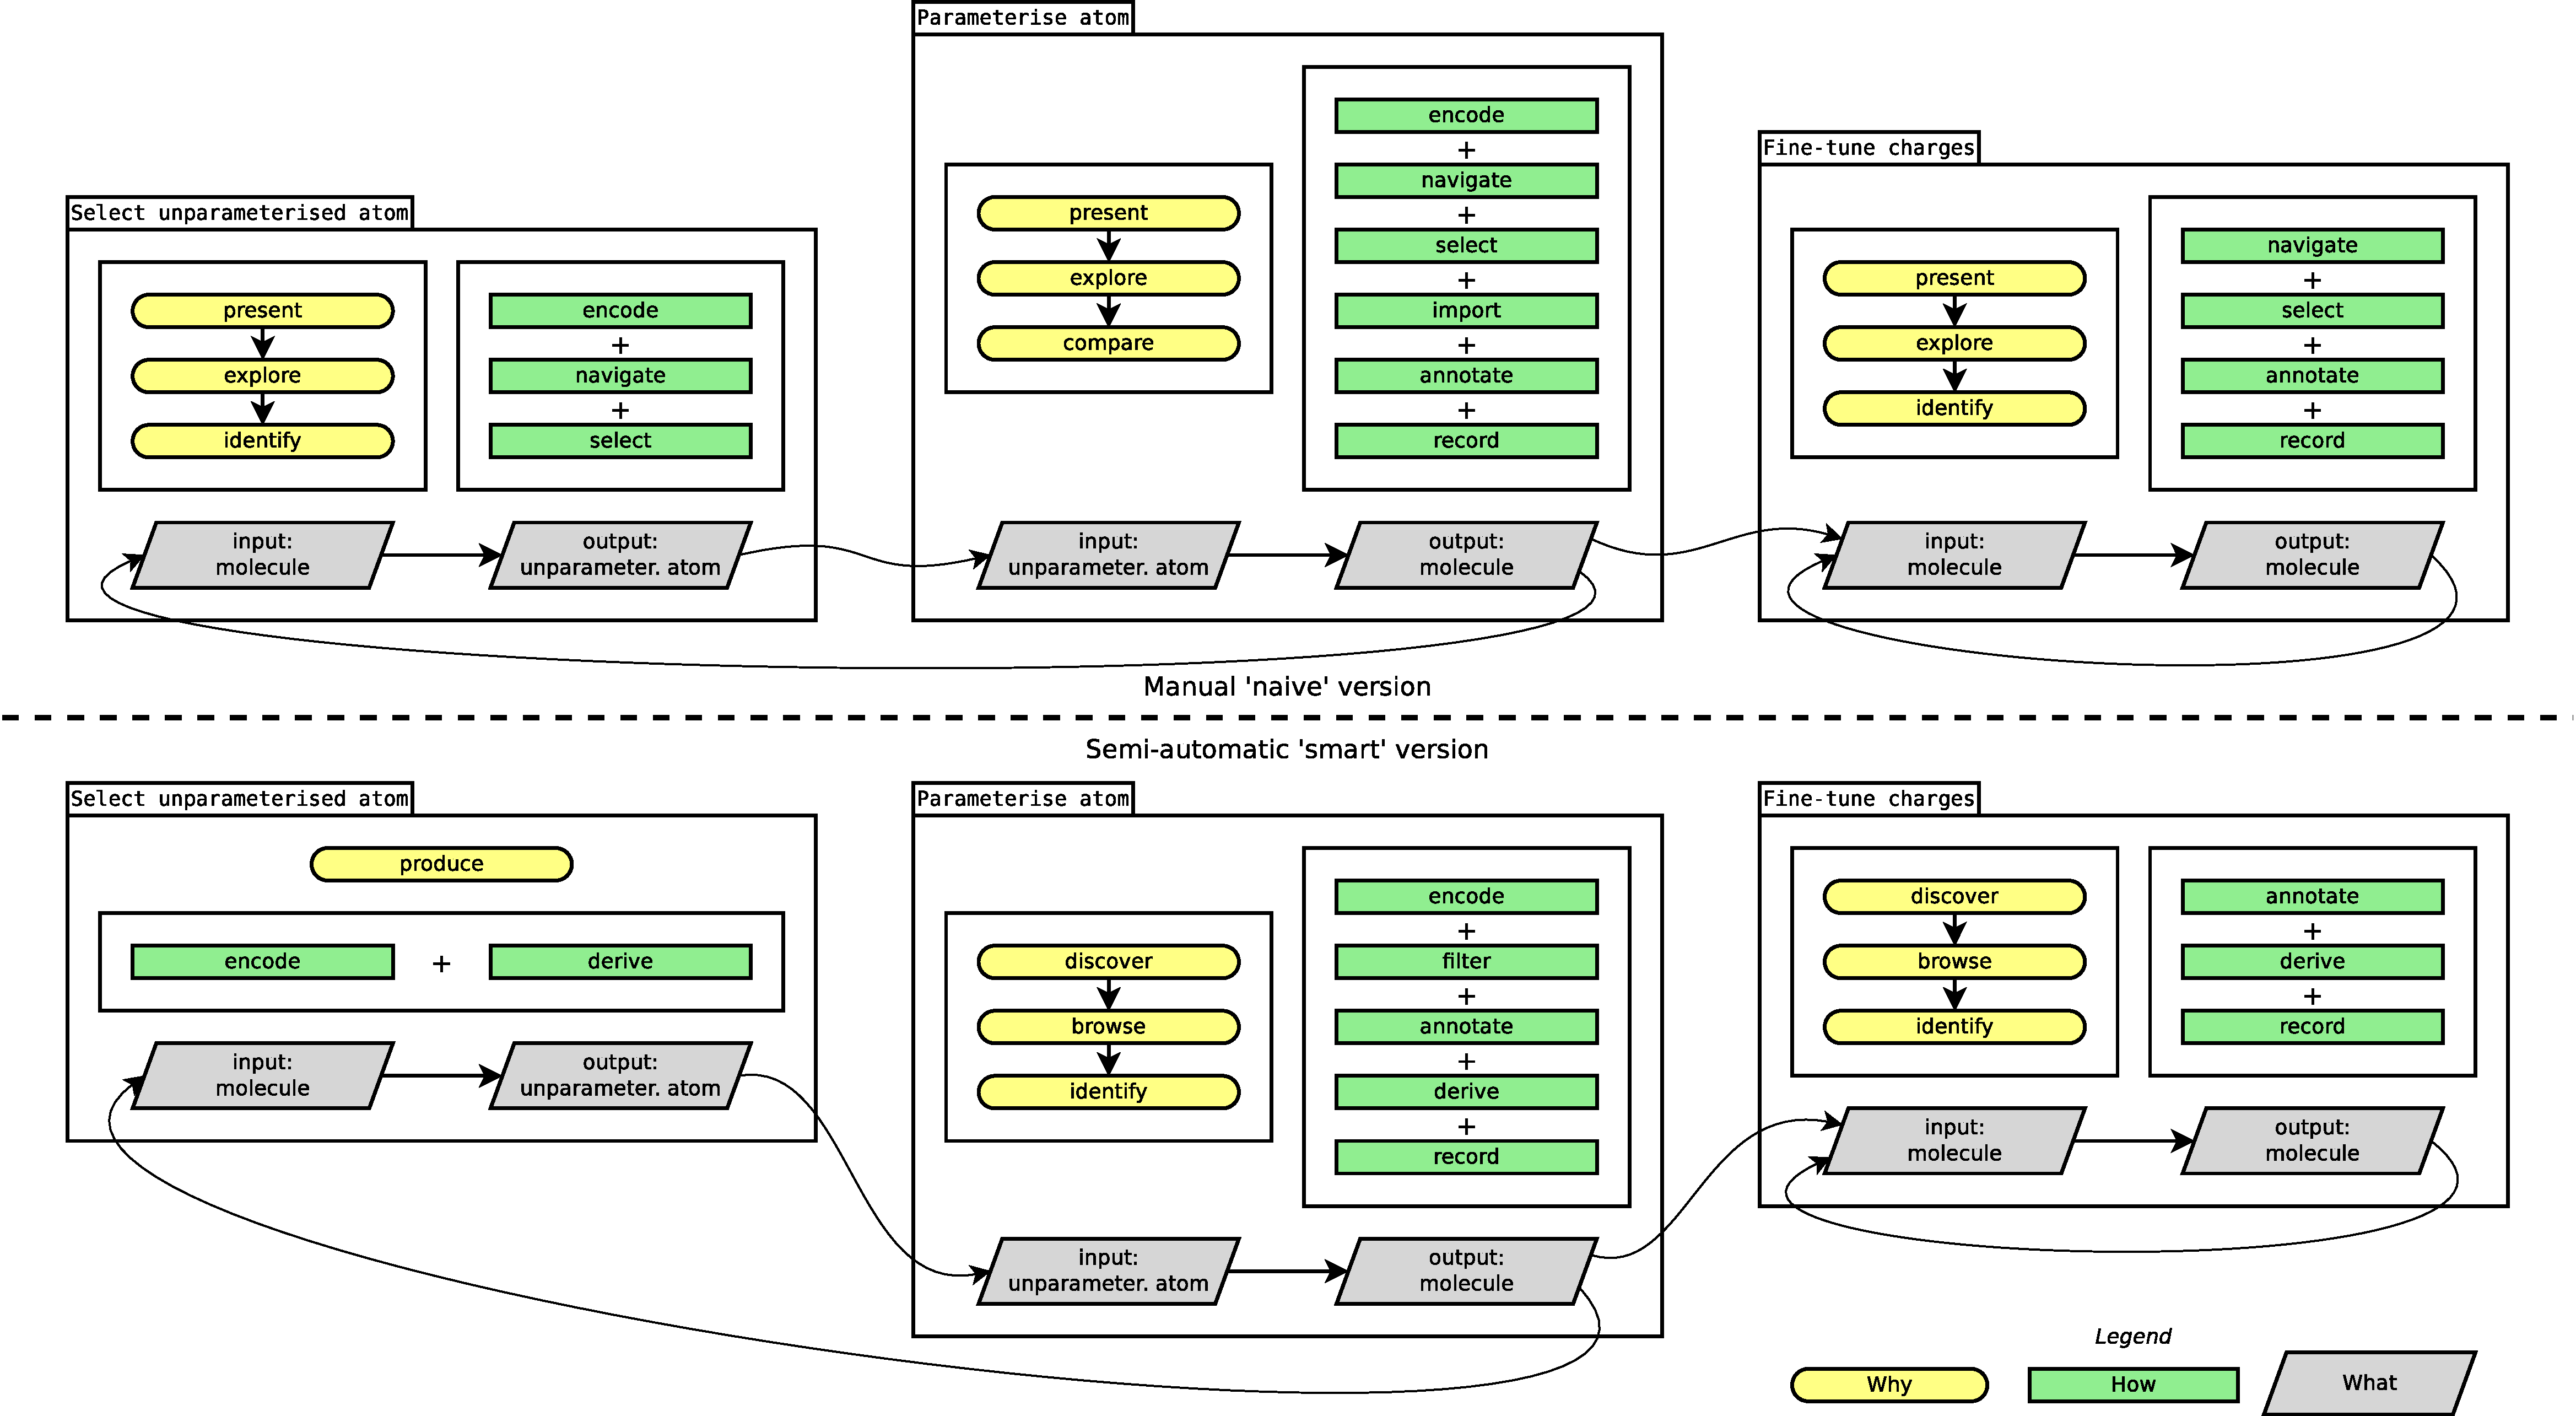
\includegraphics[width=\textwidth]{img/complete_typology.pdf}
\caption{Brehmer-Munzner Typologies of the two different interaction designs.}
\figlab{id_typologies}
\end{center}
\end{sidewaysfigure}

Blah blah these differences, blah blah one is better, blah blah because I say so\ldots


\section{Evaluation}
\seclab{evaluation}

To evaluate the project, both versions of the developed tool will be subjected to a number of user studies. Currently, however, the presumed user base is limited to only a small number of researchers. Luckily, project supervisors Klau and El-Kebir keep a close connection with most of those researchers, who work at VU University Amsterdam. They have shown some interest in the tool and are willing to participate in the user studies. Furthermore, as some of the researchers are also teaching, they can ask some of their students to evaluate the tool as well. This way, it is still possible to find enough test subjects, despite the fact that, initially, there are only a few targeted users.

In the user studies, the test subjects will be split up in two groups, where each subject is randomly assigned to a group and both groups are of equal size. One group will evaluate the naive version of the tool, the other will do the same for the smart version. Each group member will be asked to parameterise a few molecules of increasing size and complexity. The first one will be quite easy to complete, but the last one should be of such complexity that, theoretically, using the tool is beneficial over using conventional quantum mechanical calculations. It is in these last situations that the tool should show its true value.

During the tasks, the time required to complete the parameterisation will be measured. The difference between the time required in the two implementations will help deciding which of the two implementations is better, but, for both tools, completing the parameterisation should definitely not take hours to finish. Furthermore, users should never be annoyed or willing to stop parameterising.

Besides time, the user will also be scored on his performance. In order to do this, the molecules that the user will be asked to parameterise should already have been parameterised using the conventional quantum mechanical calculations. This way, the user's results can be compared to the outcomes of the calculations to establish his score. The smaller the difference between the two, the better the performance of the user will be graded. Of course, there will always be a small difference between the manual and calculated ways, as the manual assignment cannot be as precise as the calculated one is. However, as long as the difference is small, the developed tool can be considered useful to speed up atomic charge assignment.

After completing their tasks, the users will be asked to answer a number of questions about the tool. These will mainly be about how they like the design and if they can see themselves using it, but will also ask them for suggestions on things that can be improved or added. This way, their experiences can be used to further improve the tool, and to make it a tool they really like using.


\section{Time line}
\seclab{timeline}

There is a period of five months available for this project, which will be spent as follows:

\noindent
\begin{tabular}{r|l}
\textbf{Sep-Nov} & Project plan and literature study\\
\textbf{Oct-Jan} & Iteratively design, implement and validate the tool\\
\textbf{Jan-Feb} & Thesis\\
\textbf{Feb} & Thesis defence
\end{tabular}

\noindent
Note that in September and October, the project will only be worked on three days per week. From November to January, the project will be worked on full time.

User studies with real potential application users will hopefully be held in the second half of December, but might, due to the holidays, be delayed to the first half of January. Having the user studies before the end of the implementation phase allows for an additional period in which any flaws discovered by the user studies can be fixed. However, this also means there should be a working version of the tool before the end of December. During the implementation phase, frequent progress meetings with the project supervisors will be organised, to make sure flaws are discovered at an early stage and can be quickly solved. This takes away the need for a testing, fixing and improving phase at the end of the project.

\chapter[Expected results]{Expected results of the project}
Give an explicit list of all the results that are expected from the project. 

\lipsum[16]

\chapter{System requirements}
\chlab{requirements}

In order to be able to run \oframp, certain system requirements need to be met. We discuss the requirements for both the user (\secref{client_req}) and the servers (\secref{server_req}) in this chapter.


\vspace{-.1cm}
\section{Client requirements}
\seclab{client_req}
In order to be able to use \oframp, a modern browser needs to be used. There are no hardware requirements, other than those of the browser that is used to access the system. We provide support for the following browsers:

\lfootnotetext{chrome}{\url{http://chrome.google.com/}}
\lfootnotetext{ie}{\url{http://windows.microsoft.com/en-us/internet-explorer/download-ie}}
\lfootnotetext{firefox}{\url{http://www.mozilla.org/firefox/‎}}
\lfootnotetext{opera}{\url{http://www.opera.com/download‎}}
\lfootnotetext{safari}{\url{http://support.apple.com/downloads/\#safari}}

\noindent
\begin{minipage}[t]{0.5\textwidth}
\textbf{Partially supported browsers}:\vspace{.5em}

\begin{tabular}{|l|l|}
\hline
\textbf{Browser name} & \textbf{Min. version} \\\hline
Google Chrome\lfootnoteref{chrome} & 1 \\\hline
Internet Explorer\lfootnoteref{ie} & 7 \\\hline
Mozilla Firefox\lfootnoteref{firefox} & 4 \\\hline
Opera\lfootnoteref{opera} & 12 \\\hline
Safari\lfootnoteref{safari} & 5 \\\hline
\end{tabular}
\end{minipage}
\begin{minipage}[t]{0.5\textwidth}
\textbf{Fully supported browsers}:\vspace{.5em}

\begin{tabular}{|l|l|}
\hline
\textbf{Browser name} & \textbf{Min. version} \\\hline
Google Chrome\lfootnoteref{chrome} & 25 \\\hline
Internet Explorer\lfootnoteref{ie} & 10 \\\hline
Mozilla Firefox\lfootnoteref{firefox} & 25 \\\hline
- & - \\\hline
Safari\lfootnoteref{safari} & 7 \\\hline
\end{tabular}
\end{minipage}

Note that no version of the Opera\lfootnoteref{opera} browser is full supported. This is currently not possible due to the fact that, in that browser, mouse gestures are automatically bound to right mouse click and drag actions. As, in \oframp, these actions are used to make multi-atom selections, it is not possible to provide complete support for the Opera browser.

The system has been mostly tested and implemented using Google Chrome\lfootnoteref{chrome}. It is therefore recommended to use the latest version of that browser, in order to get the best experience.



\section{Server requirements}
\seclab{server_req}
As discussed before, \oframp{} consists of three systems: \oapoc{} for retrieving the atom positions, \omfraf{} for getting the fragments, and \oframp{} itself, which is the web service the user connects to. For the best results, it is advised to run all of these systems on separate servers, as both \oapoc{} and \omfraf{} have to perform computationally intensive tasks.

For \oframp, it is not necessary to be run on a server with very high performance. This server basically only needs to serve two \verb|HTML| pages, a few images, and some \verb|CSS| and \verb|JavaScript| files. \oapoc{} and \omfraf, on the other hand, are a different story, as they perform tasks that are both computationally and memory-wise intensive. Even though the processes are currently not parallelised, running the systems on multi-core machines will help with simultaneous processing of multiple users.

\lfootnotetext{oapoc_only}{Only for \oapoc}
\lfootnotetext{omfraf_only}{Only for \omfraf}

\noindent
\begin{table}[h!]
\begin{center}
\begin{tabular}{|p{.45\linewidth}|p{.45\linewidth}|}
\hline
\oframp & \oapoc / \omfraf \\\hline
Simple web server & Good web server \\
Single-core & Multi-core w/ high single-thread performance \\
100MB RAM & 1GB RAM \\
Apache (or similar) & Apache (or similar) \\
PHP 4 (or newer) & Python 2.7 \\
 & Django 1.4 \\
 & Open Babel 2.3.2\lfootnoteref{oapoc_only} \\
 & LEMON Graph Library 1.3\lfootnoteref{omfraf_only} \\\hline
\end{tabular}
\end{center}
\caption{Requirements for the different systems.}
\label{server_req}
\end{table}

Table~\ref{server_req} shows the requirements for the different servers. Note that a different configuration with a simpler server for \oapoc{} or \omfraf{} may also work, but might not give the desired performance. Furthermore, different software versions might work as well, but have not been tested.

\chapter{Risks}
\chlab{risks}

Just like every other research project, this project does not come without risks. In this chapter, the risks that come with this project will be discussed, along with possible counter measures.

\begin{description}
\item[Limited knowledge about chemistry]~~\\
It does not seem that thorough understanding of chemistry is really needed for this project. If, however, it turns out that at some point more in-depth chemistry knowledge is needed, the supervisors of this project have agreed to help solving the chemistry related problems.

\item[Molecule section matching algorithm is still being developed]~~\\
Besides repeatedly asking people to finish something, there is not much you can do to make sure something others are developing will be done in time. A workaround for this problem would be to temporarily use a fixed, static set of molecule sections. These sections may or may not be related to the molecule that is being analysed, but al least this allows for almost complete development of the application without being dependent on the work of others.

\item[Existing tools may not be easily extendible]~~\\
If the existing molecule drawing applications turn out to be unextendible, the visualisation of the molecules will have to be implemented from scratch. Luckily, there are some open source graph drawing libraries for \verb|JavaScript|, e.g. \verb|D3.js|~\cite{bostock2012data}, \verb|Raphael.js|~\cite{baranovski2013raphael} and \verb|JavaScript Graph Library|~\cite{dracula2012javascript}. These libraries reduce the complexity from having to implement a whole drawing system to restricting an existing drawing system such that it will correctly draw molecules. 

\item[No real comparable tools exist]~~\\
As there are no existing tools for fragment-based molecule parameterisation, it is unknown what will be a good way of doing this. To mitigate this risk, frequent meetings with the project supervisors will be organised to ensure flaws are discovered in an early phase.
\end{description}

\chapter{Literature survey}
\chlab{literature}

For this research project, quite a lot of literature is available. The literature has been organised into four different categories, for each of which a number of papers will be discussed.


\section{Molecule simulations}
\seclab{simulations}

Canzar and El-Kebir discuss their work on charge group partitioning~\cite{canzar2012charge}. They explain what is needed for running biomolecular simulations and in which steps this information can be gathered. When the atom types, bonds and partial charges of a molecule are known, calculating the charge groups allows for running biomolecular simulations on very small time scales, while still being precise. $\mathcal{NP}$-hardness of the partitioning problem is proven, and an algorithm for quickly calculating the charge groups is presented. The proposed research project is not about assigning charge groups, but the work of Canzar and El-Kebir shows the need for finding the atomic partial charges of a molecule. It also indicates where in the process the partial charges should be calculated, and what will be done with them afterwards.

Malde et al. present the Automated Force Field Topology Builder~(ATB)~\cite{malde2011automated}. The ATB is a web service that can provide topologies for use in molecular simulations. It can both act as a repository for already parameterised molecules and it is able to parameterise molecules itself. This automatic parameterisation is done using some quantum mechanical calculations, which are very complex and computationally intensive. In the proposed research project, an attempt is made to improve the calculations of atomic partial charges. The results obtained by the tool to be developed will be compared to those obtained by the ATB, in order to validate the value of new tool.


\section{Interaction design}
\seclab{design}

Besides trying to optimise the preparation steps for molecule simulations, the main challenge of this research project is to come up with a good interaction design for a tool that does that. In the interaction design area, Donald Norman is a respected and often cited author. He feels that technology can only live up to its full potential by, first of all, supporting human tasks, while making the supporting technology as transparent as possible by making the tools easy to use, easy to learn and easy to understand. Designing for this purpose is called user-centred design~\cite{norman2002design}.

One of the most important aspects of design is visibility. Every interface should have visible features that can send the right messages to the user. It is very important that a user's actions do not have coincidental consequences. Otherwise, the user can develop wrong expectations of his actions, which may later result in problems while using the tool. What is also important, is that if a user does make a mistake, he should be able to undo this. If this is \emph{not} possible, he may get easily frustrated and will stop using the tool. Finally, the user may not get lost in an enormous list of features. As many of these features will often rarely be used, tools with less features are often the better ones.

An often occurring problem with interfaces is that they get in the way of the task that needs to be performed~\cite{norman1990interfaces}. The user of a tool should not be spending his time `using the interface', but rather on performing the task the tool is supposed to help him with. In order to achieve this, product design should start with analysing the user and the task, and only then designing the user interaction.

When doing interaction design, one has to keep in mind that the appearance of a tool can have a great impact on how well the user of that tool can carry out the tasks the tool is intended for~\cite{norman2002emotion}. Tools that look unattractive tend to focus the mind, which leads to better concentration. For tasks where something needs to be done quickly, this is good, but in cases where creative thinking is required, this will not provide a satisfying result. In that case, the thought processes should be broadened by having something that looks really good. This can easily get the user distracted, which allows for creative thinking.

In an attempt to overcome the poor design of many software products, an approach called human-centred design (HCD) has been developed~\cite{norman2005human}. However, even though the needs of the user play a central role here, many companies following the HCD principles still develop complex and confusing products. The systems are often superb at the level of the static, individual display, but fail to support the sequential requirements of the underlying tasks and activities. Therefore, a new approach is needed that does not put the user in a central role, but rather does so with the activity that needs to be performed. In this activity-centred design method, it is sometimes necessary to ignore a user's requests as they might compromise the task that has to be carried out.

This, however, does not mean that the application user's needs should be completely ignored. On the contrary, it is really important that the user's characteristics are understood and used in the design of an application~\cite{badre2002shaping}. Also, a good analysis of the context is needed to make the right design decisions. If one ignores the user characteristics and context of an application, the application is  likely to fail, as the context in which the application is developed will almost always differ from the context in which it will be used.

Following the previously discussed and other research, a number of principles of interaction design can be identified. However, different authors have different opinions on what those principles are. Norman and Nielsen identify the following principles of interaction design that are completely independent of technology~\cite{norman2010gestural}:
\begin{itemize}[noitemsep,topsep=0pt,parsep=0pt,partopsep=0pt]
\item Visibility (also called perceived affordances or signifiers);
\item Feedback;
\item Consistency (also known as standards);
\item Non-destructive operations (hence the importance of undo);
\item Discoverability: all operations can be discovered by systematic exploration of menus;
\item Scalability: the operation should work on all screen sizes, small and large;
\item Reliability: operations should work and events should not happen randomly.
\end{itemize}
Thimbleby, on the other hand, \emph{does} relate his principles to technology~\cite{thimbleby2007press}:
\begin{itemize}[noitemsep,topsep=0pt,parsep=0pt,partopsep=0pt]
\item Use good algorithms for better user interfaces: interactive devices are designed to solve problems in a structured way, which is exactly what a good algorithm does;
\item Use simple, explicit interaction frameworks: those provide clear interaction structures, which allow for reliable feature integration, checking, analysis, fault identification, and error fixing;
\item Interrelate all interaction programming: all aspects of the design should come out of the same specification;
\item Define properties and analyse designs for them.
\end{itemize}
A more extensive list is provided by Blair-Early and Zender~\cite{blair2008user}:
\begin{itemize}[noitemsep,topsep=0pt,parsep=0pt,partopsep=0pt]
\item Obvious start: design an obvious starting point;
\item Clear reverse: design an obvious exit or stop;
\item Consistent logic: design an internally consistent logic for content, actions, and effects (the most important consistency is that with user expectations);
\item Observe conventions: identify and consider the impact of familiar interface conventions;
\item Feedback: design tangible responses to apt user actions;
\item Landmarks: design landmarks as a reference for context;
\item Proximity: design interface elements in consistent proximity to their content objects and to each other;
\item Adaptation: design an interface that adapts or is adapted to use;
\item Help: as necessary, provide a readily accessible overall mechanism for assistance;
\item Interface is content: design interface elements that minimise interface and maximise content.
\end{itemize}


\section{Molecule software}
\seclab{software}

There is a lot of available software for displaying, drawing and editing molecules. These programs form an indispensable part of every molecular processing system~\cite{ertl2010molecular}. Throughout the years, these programs have evolved from basic text editors, through clickable image maps, to full-on molecular structure sketching software. In the last few years, a new trend becomes visible. More and more cheminformatics applications are being brought to the web, allowing for a lot of new ways of interaction. Furthermore, these new applications are being open sourced, allowing for new innovative variations or combinations of the old tools.

An example of a previously offline, closed source tool is \verb|JSmol|, previously known as just \verb|Jmol|~\cite{hanson2013jsmol}. This tool has been seamlessly transformed from a \verb|Java| applet to \verb|JavaScript|, without any visible visual difference. Furthermore, performance wise, there is only a minor difference between the two implementations. Another example is \verb|JSME|~\cite{bienfait2013jsme}. This tool has even been cross-compiled from its original \verb|Java| code to \verb|JavaScript| using the \verb|Google Web Toolkit| compiler. The transition to the web has resulted in the addition of several features, suggested by users from the new, bigger audience. What can be concluded from these two cases is that bringing molecule software to the web opens up a whole world of new possibilities, without having to give up on performance.

With the ongoing migration of molecule software to the web, new devices, such as smartphones and tablets, will be able to run the tools. As these devices promote different ways of user interaction and often have smaller screens, designs of the molecule software need to be reconsidered. \verb|TB Mobile| is a mobile app for identification of potential anti-tuberculosis molecules~\cite{ekins2013tb}. The app is structured in such way that there is always a small control bar at the top, and a large area for showing the content. Interaction with the app is handled by a small number of large buttons, allowing for easy touch controls. In order to work for different screen sizes, everything in the content area is scalable, and, in case not everything fits on the screen, scrollable. Usage of the app in practice has shown that it helps to improve the work flow of tuberculosis researchers, by lowering the barriers for accessing the information it provides.

The issue of showing a lot of data on a limited-size screen is also addressed by Ertl and Rohde~\cite{ertl2012molecule}. They took the concept of a word cloud, and transformed that to a molecule cloud, where the highest scored molecules are the biggest and the lowest are the smallest. None of the molecules overlap, and the sizes are divided such that the whole available screen space is filled. User studies have shown that these molecule clouds provide an easy way of finding the most relevant molecules. In the proposed research project, this may be useful for showing the set of related sections of other molecules, depending on the size of that set.


\section{Molecule data formats}
\seclab{data_formats}

For importing, storing, and exchanging molecule structure data, various formats exist. One of these formats is \verb|SMILES|, a very minimal line notation for molecule structure data~\cite{daylight1992daylight}. Back in 1988, when \verb|SMILES| was first introduced, it was quite common to store molecular structures as connection tables. These tables took a lot of storage space and were not easily exchangeable, so something new needed to be developed. The \verb|SMILES| representation of a molecule is just a simple linguistic construct that uses a simple vocabulary for atom an bond symbols. It has remained popular since then, and is still used in many molecule editors today.

Nevertheless, attempts have been made to replace the \verb|SMILES| format, as it is a closed standard with only limited possibilities. In 2005, a new format called \verb|IUPAC InChI| was introduced~\cite{heller2013inchi}. \verb|InChI| is an open format that aims to combine chemical, biological and other related information in a single representation. Still being a linguistic representation like \verb|SMILES|, it is easily exchangeable and allows for simple machine processing. In the past few years, \verb|InChI| has become the international, worldwide standard for defined chemical structures. As \verb|SMILES| is also still widely used, the tool that will be developed in the proposed research project will support both the \verb|SMILES| and \verb|InChI| formats for entering molecules into the system.


\bibliographystyle{abbrv-rt}
\nocite{*}
\bibliography{references}
\chaptermark{Bibliography}

\appendix

%\include{something}

\end{document}
